% Introduction

% ??? NEED block diagram of go()! check map? scan: yes/no? save map, move etc. (use that online code to block diagram tool)
% ??? Descripe framework in a section (see gdocs for input to block diagram) (or present at exam)
% ??? Mention we chose to focus on making our own code with the least use of finished libraries as possible, no error handling 
% ??? Mention the report will explain important aspects of out work and theoretical parts, 
%     while the finished product is a prototype and the code in the appendix
% 

% Problem / introduction?:
% - Problem and analysis:
% 	- https://en.wikipedia.org/wiki/Rescue_robot
%	- https://www.robocupgermanopen.de/sites/default/files/rescue_maze_2017.pdf
% - System diagram (what we want to build):
% Daniel has already made a nice diagram of this
% Current position should be known after each move.

% - Prototype / mechanical design / robot design (show what we wanted to to build)
% - maybe here with motor/wheels under it? chasis?
% - maybe under "problem and analysis"


% Programming Structure and Design: (try to fulfill some Akbar goals here, see those gdocs notes)
%- Robot Instruction Execution Order
%- Framework
%- Data Structure



% Robot control: (maybe after pathfinding?)
% Theory:
% - functionality
% - step/control sequence
% Implementation: (programming)
% - programming/framework etc.

% Map handling:
% Theory (how we did and thoughts):
% - Introduction (what is map handling about, what have we covered here, problems we want to solve)
% - Analysis of map input
% - Converting analog map to digital map (intro)
% - 
% Implementation:
% - Read, compare, update 

% Prototype:
% maybe something about the prototype here??
% or in conclusion at least
% read google docs



\chapter{Map Handling}
\label{ch:map_handling} % chapter label
The rescue robot should be able follow a given path from start to finish, based on a predefined map given as input.
A map provides useful information about whether areas of the map are accessible or not. Map data can be loaded by the robot prior to its physical presence at a location. Once the robot is at the starting point, it has to rely on its sensors for updated information about the surroundings. 

The map itself is a crucial part, that converted into to a graph is used by the path-finding as explained in Chapter \ref{ch:path}. Hence a structured way of storing the required map data for different maps was designed. The primary goal was make it readable by the microcontroller, but also still allow easy user input.

%Existing pathfinding algorithms such as Dijkstra and A* was studied, 
%in order to understand what input data such algorithms typically would require. 
%The pathfinding algorihtm implemented in this project is further described in chapter \ref{ch:path}.

\newpage
\section{Map Requirements}
\label{sec:map_requirements}
Maps can be found in a lot of different styles,
varying in how they represent specific informations.
Those styles often depend on the purpose of the map.
Figure \ref{sub:orient} shows a map for casual orientation purposes,
while \ref{sub:evac} shows a standardized evacuation plan.

\begin{figure}[h!tp]
    \centering
    \subfloat[Section of AAU Esbjerg]{%
        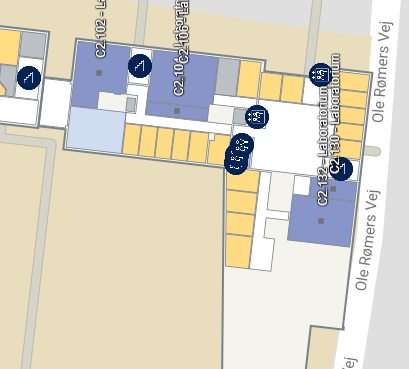
\includegraphics[width=0.4\textwidth]{figures/map/floorplan_aau.png}%
        \label{sub:orient}
        }%
    \hspace{0.1\textwidth}
    \subfloat[School layout example]{%
        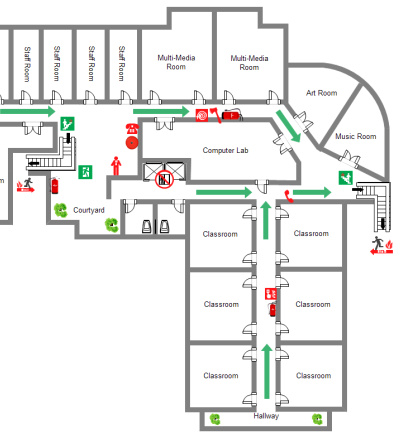
\includegraphics[width=0.4\textwidth]{figures/map/floorplan_school.png}%
        \label{sub:evac}
        }%
    \caption{Examples of different maps}
    \label{fig:floor_plans}
\end{figure}
% https://www.edrawsoft.com/school-layout-example.php

Maps are often very visual, providing a lot of detailed information to the reader.
The way the information is represented differently,
makes it very hard to be interpreted automatically.
A map must provide necessary information,
in a way that can be interpreted by the micro controller.
For this project we decided that a simplified map, would be sufficient.

Table \ref{table:map_data} shows the data the map should include,
as well as some areas that have been delimited from.

\begin{table}[h!]
	\centering
	\caption{Map data}
	\begin{tabular}{|p{0.4\textwidth}||p{0.4\textwidth}|}
		\hline
		Data to be included & Data to delimit from \\ 
		\hline
		Map dimensions 		& \parbox[t]{0.4\textwidth}{Differences in height\\(levels, stairs etc.)}\\
		\hline
		Start position 		& Door openings \\
		\hline
		Finish position 	& \parbox[t]{0.4\textwidth}{Ground surface\\(slipping, traction)} \\
		\hline
		Walls 				& Objects\\
		\hline
	\end{tabular}
	\label{table:map_data}
\end{table}

\section{Map Coordinates}
\label{sec:map_coordinates} % section label
During the theoretical development we often used hand-drawn 2D maps with grids as depicted in Figure \ref{sub:2d_map}. 
The map can have a certain size and allows for an object such as a wall to have a location on the grid. 
A specific part of the map can easily be referred to by its unique coordinate in the x and y dimensions. 

For converting and storing analog maps into a usable digital representation with the same properties, 
we chose to use a 2D array as data structure. 
A 2D array can be thought of as a matrix, where a grid of numbers can be arranged in rows and columns. 
2D arrays are very similar to matrices, and differs in how elements are indexed.

The result of the different indexing methods can be seen by comparing Figure \ref{sub:2d_map} to \ref{sub:2d_array}. 
Given the same index values, the cell referred to would be different, 
as seen in  Figure \ref{sub:2d_map} and \ref{sub:2d_array}.


\begin{figure}[htp]
    \centering
    \subfloat[2D grid map]{%
        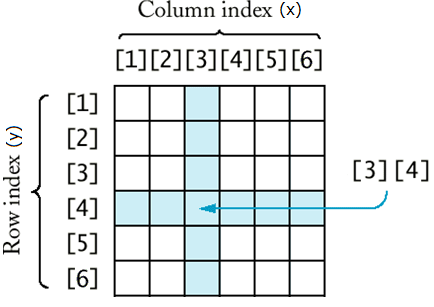
\includegraphics[width=0.45\textwidth]{figures/map/2d-map.png}%
        \label{sub:2d_map}
        }%  
    \hspace{0.05\textwidth}  
    \subfloat[2D array]{%
        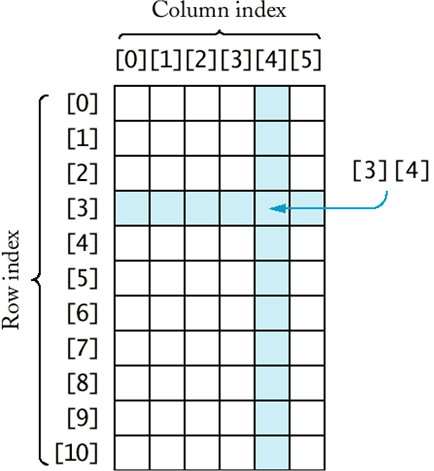
\includegraphics[width=0.45\textwidth]{figures/map/2d-array.png}%
        \label{sub:2d_array}
        }%
    \caption{Difference in indexing for (3,4) in a 2D grid map and a 2D array}
    \label{fig:floor_plans}
\end{figure}
%https://i.stack.imgur.com/tFdLk.gif

Each cell in the map represents a map segment with its own set of coordinates. 
We chose to start map coordinates at zero, and had the option to switch rows and columns if needed, 
which is similar to a matrix transpose. 
This could be done in the syntax by switching i and j, 
or by switching the x and y axes when storing the map in the first place.
\\

\begin{lstlisting}[caption={Example of map segment before rows and columns are switched}]
Array: map[4][3], would give map coordinate (3,4)
\end{lstlisting}

\begin{lstlisting}[caption={Example of map segment after switching rows and columns}]
Array: map[3][4], would give map coordinate (3,4)
\end{lstlisting}

This lead to the final implementation in our program using dynamic 2D arrays, 
where the value of any given map segment easily could be accessed. 
\\
\begin{lstlisting}[caption={Example of implementation in the final code}]
Array: robot->map->segments[3][4], would return the value for map coordinate (3,4)
\end{lstlisting}
Examples of this can be seen implemented in the final code in appendix XX (some specific place?). 
\todo{fix referring to code in appendix, and code language should not be set to Python.} 
The same approach was used for handling node maps, which is further explained in Chapter \ref{ch:path}.

\newpage

\section{Map Design}
\label{sec:map_design} % section label
The grid-based map is made up of simple plain-text ASCII characters.
This makes it fairly simple and easy-to-understand, and maps can easily be created or changed by a user. 

An example of a map with 5x5 nodes can be seen in Figure \ref{sub:map_ascii}, where \# being walls, A being the start, B being the finish, o being nodes, and the white spaces being open spaces. The same map can be seen using UTF8 encoding in Figure \ref{sub:map_utf8}. UTF8 has a more characters to choose from, which makes it easier to read for humans while the plain-text version is easier to read for computers.

Nodes represent positions on the map where the robot can move between. The robot can move in any of the eight directions unless a it is blocked by a wall. The directions consists of four straight directions, N,E,S,W and four diagonal directions NE,SE,SW,NW. Nodes are explained further in Chapter \ref{ch:path}. \todo{explained in path chapter or in nodemap section?}

\begin{figure}[htp]
    \centering
    \subfloat[ASCII]{%
        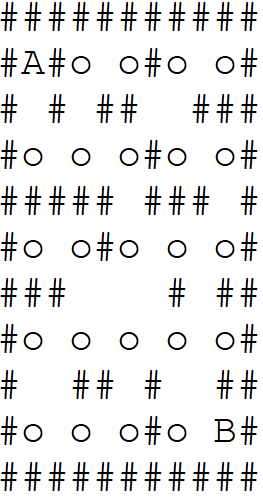
\includegraphics[width=0.2\textwidth]{figures/map/5x5map_ascii-2.png}%
        \label{sub:map_ascii}

    }
    \hspace{0.2\textwidth}
    \subfloat[UTF8]{%
        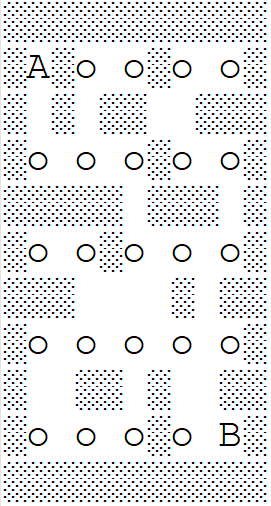
\includegraphics[width=0.2\textwidth]{figures/map/5x5map_utf8-2.png}%
        \label{sub:map_utf8}
    }
    \caption{Example of a map with 5x5 nodes, having 11 characters per line and 11 lines.}
    \label{fig:5x5map}
\end{figure}

We found that making the map using UTF8 would require a bit more work, since text editors often add characters to the beginning of the file. 
This is known as the byte-order-mark (BOM) which indicates the file uses UTF8 encoding. 
It also uses variable bit-length for characters, between 1-4 bytes [https://en.wikipedia.org/wiki/UTF-8].
\todo{not wikipedia PLEASE!!} 
This makes reading and storing the map to a file more complicated, which is why we chose to use plain text ASCII.

\newpage
\section{Reading Map from a File}
\label{sec:map_read} % section label %
The function {\tt map\_load} loads map data from a file and saves it in the {\tt map} struct.
Start and finish positions are read from the file as well, and saved in {\tt robot} struct.
\todo{Write about structs in the beginning of the report}

Functions were made for loading maps from a text-file, as well as saving an updated map to a text-file. 
The full code for the functions {\tt map\_load} and {\tt map\_save} can be seen in Appendix X.\todo{fix reference}
\todo[inline]{listing showing parts of these functions}
Reading and writing maps on a computer locally, was very useful for developing and testing the map handling subsystem. 
Implementing this functionality on a microprocessor, would require it to have a file system installed.
We chose not to implement this functionality, due to the restricted time frame of this project.
As an alternative, maps can be stored directly in memory as part og the programming code. 
This solution is not as user-friendly, and updates to the map will be lost from the memory when the microcontroller is turned off.

\todo[inline]{something in between, maybe some code?}
In the C programming language the size of an array must be declared at compile time. 
The array for the map has to be large enough to hold all the map data.
Unfortunately the map size and data remains unknown until a map is loaded, which happens at runtime.

One way of dealing with this, is by using a 2D array with a fixed size, large enough to store maps of a convenient size. 
We chose to use a dynamic 2D array instead. This more advanced approach would give us more experience, by using dynamic memory allocation and pointers to implement this solution in the application.

The required size of the dynamiic 2D array can be calculated by counting the lines and characters of the map,
which is equivalent to the rows and columns needed for the array.
A map with 5x5 nodes will have 11 characters in each line and a total of 11 lines,
as illustrated in Figure \ref{fig:5x5map}.
To store the map, an 11x11 2D array is required.
Now that the required array size is known, it can be allocated in the memory.\\
\todo[inline]{insert code}
- Example of allocating 2d array\\
- putting data in 2d array ???\\

ORDER:\\
map load\\
hex values\\
node map load\\
scan\\
map save


\section{Encoding Walls in a Single-byte Value}
\label{sec:map_hex} % section label
Each node in the map potentially has up to eight neighbour nodes. 
The robot can move to any of the neighbour nodes, unless it is blocked by a wall, as illustrated in Figure \ref{fig:node_move_directions}.\todo{insert figure of a node and 8 arrows}

To indicate the possible directions to move in, we decided to use the boolean values 0 and 1. 
Here 0 would mean it is possible to move that direction to the neighbour node, while 1 means the direction is blocked by a wall.

Since each 0 or 1 can be represented by one bit, it is possible to store data about all eight directions in a single byte.
byte --> [0000 0000] \todo{insert figure or table here as an example?}

Depending on the individual bits, the byte will have a certain value.
Since all values are stored as binaries in the memory, a hexadecimal representation was often used in the programming.

\todo{merge this section with Daniels 5.7 Implementation}


\section{Building a Node Map}
\label{sec:map_node} % section label
Path finding algorithms operate with a special type of map called a graph.
A graph consists of only nodes and edges, as explained more in detail in Section \ref{sec:graphs}.

The function {\tt node\_map\_load} converts the ordinary map made of ASCII characters, into a map that only consists of nodes.
To store the node map we created the data structure {\tt Nodes struct} to hold the necessary data for a single node.
Each {\tt node struct} has pointers to the available neighbour nodes in all eight directions.
\todo{insert node struct code?}


A dynamic 2D array was filled with {\tt Nodes struct} for each node in the map was declared. 
\todo{code here?}
A pointer to the declared 2D array gets stored in the {\tt robot struct}.
This allows for easy access to all the data for a given node, just by using the nodes position on the map as the array index values.

\todo{give example}
robot->nodemap.node[i][j].[name of struct element]

\section{Map Validation Using Sensors}
\label{sec:map_check} % section label
There might be rescuing scenarios where parts of the map, or even the entire map, would be unknown.
External factors such as an explosion in a building, could also change the surroundings dramatically, making the map data invalid.
 
The robots current location on the map is known at all times. 
After the robot has moved to the next node on the map, its current position is updated.
At the robots current location, distance sensors scans the surrounding environment for walls in the eight possible move-directions.
How these sensors operate is described in more detail in Chapter \ref{ch:scan}.
The feedback from the sensors is given as a single-byte hex value, as described in Section \ref{sec:map_hex}.
\todo{explained in Scan section what the return value of the sensors is?}
The single-byte value is compared to the corresponding segments on the map.
If changes to the surroundings are detected, the map gets updated and saved to the text-file.
\todo{insert code where char map gets updated based on the scan return}

Every time a change in the map is detected, the path finding function is called
\todo{insert function name or code}. 
This calculates the most efficient path from the robots current location to the finish, using the updated map data. 
\todo{insert code from map-check function here}
\todo{could maybe be used somewhere else to explain what the robot does, if not just leave it here.}

\section{Writing Map to a File}
\label{sec:map_save} % section label
Come up with something..



